%\chapter{Introduction}

%\section{Background and Recent Research}
%\subsection{<any sub section here>}

%\subsection{Literature Survey}

%\subsubsection{<Sub-subsection title>}
%some text\cite{citation-1-name-here}, some more text

%\subsubsection{<Sub-subsection title>}
%even more text\footnote{<footnote here>}, and even more.

\section{Motivation}

This report will provide a detailed account of the processes our group
used to design and implement a database that can be used to manage
a blood donation system. Each subsection of the report will correspond to an
important feature of database design.

\begin{sloppypar}
\section{Database Schema}

\subsection{BDC EMPLOYEE}

\begin{tabular}{ | c | c | c | c | c | c | c | }
 \hline
 \underline{EMP ID} & \underline{BDC ID} & F NAME & L NAME & DESIGNATION & DATE OF JOIN & PASSWORD \\
 \hline
\end{tabular}

\subsection{BDC BLOOD AVAILABLITY}

\begin{tabular}{ | c | c | c | }
 \hline
 \underline{BDC ID} & \underline{BLOOD GROUP} & BLOOD AVAILABLE \\
 \hline
\end{tabular}

\subsection{BDC}

\begin{tabular}{ | c | c | c | c | c | }
 \hline
 \underline{BDC ID} & CONTACT NAME & PASSWORD & \underline{MGR ID} & CITY \\
 \hline
\end{tabular} \\ \\

\subsection{BDC PAYMENT INFO}

\begin{tabular}{ | c | c | c | }
 \hline
 \underline{BDC ID} & AMOUNT RECEIVED & \underline{DATE OF TRANSACTION} \\
 \hline
\end{tabular}

\subsection{DONOR}

\begin{tabular}{ | c | c | c | c | }
 \hline
 \underline{DONOR ID} & PASSWORD & BLOOD TYPE & MOBILE NUMBER \\
 \hline
\end{tabular}
\begin{tabular}{ | c | c | c | c | }
 \hline
 E-MAIL & F NAME & L NAME & CITY \\
 \hline
\end{tabular}

\subsection{RECEIVER}

\begin{tabular}{ | c | c | c | c | c | }
 \hline
 \underline{RECEIVER ID} & F NAME & L NAME & BLOOD GROUP & E MAIL \\
 \hline
\end{tabular}
\begin{tabular}{ | c | c | c | c | }
 \hline
 MOBILE NUMBER & AMOUNT REQUIRED & DATE OF REQUIREMENT & CITY \\
 \hline
\end{tabular}

\subsection{MONETARY ORGANISATION}

\begin{tabular}{ | c | c | c | c | }
 \hline
 \underline{ORG ID} & ORG NAME & CONTACT NAME & E MAIL \\
 \hline
\end{tabular}
\begin{tabular}{ | c | c | }
 \hline
 PASSWORD & CONTACT NUMBER \\
 \hline
\end{tabular} \\ \\

\subsection{ORGANISATION PAYMENT INFO}

\begin{tabular}{ | c | c | c | }
 \hline
 \underline{ORG ID} & PAYMENT GIVEN & \underline{DATE OF TRANSACTION} \\
 \hline
\end{tabular}

\subsection{RAKTHADATHA}

\begin{tabular}{ | c | c | c | }
 \hline
 \underline{ADMIN ID} & PASSWORD & CITY \\
 \hline
\end{tabular}

\subsection{TRANSFER INFO}

\begin{tabular}{ | c | c | c |}
 \hline
 \underline{ORG ID} & \underline{BDC ID} & AMOUNT TRANSFERED \\
 \hline
\end{tabular}

\subsection{CITY - STATE}

\begin{tabular}{ | c | c | }
 \hline
 \underline{CITY} & STATE \\
 \hline
\end{tabular}

\subsection{STATE - COUNTRY}

\begin{tabular}{ | c | c | }
 \hline
 \underline{STATE} & COUNTRY \\
 \hline
\end{tabular}
\end{sloppypar}

\section{Entity Relationship Diagram}
\begin{figure}[htb]
\centering
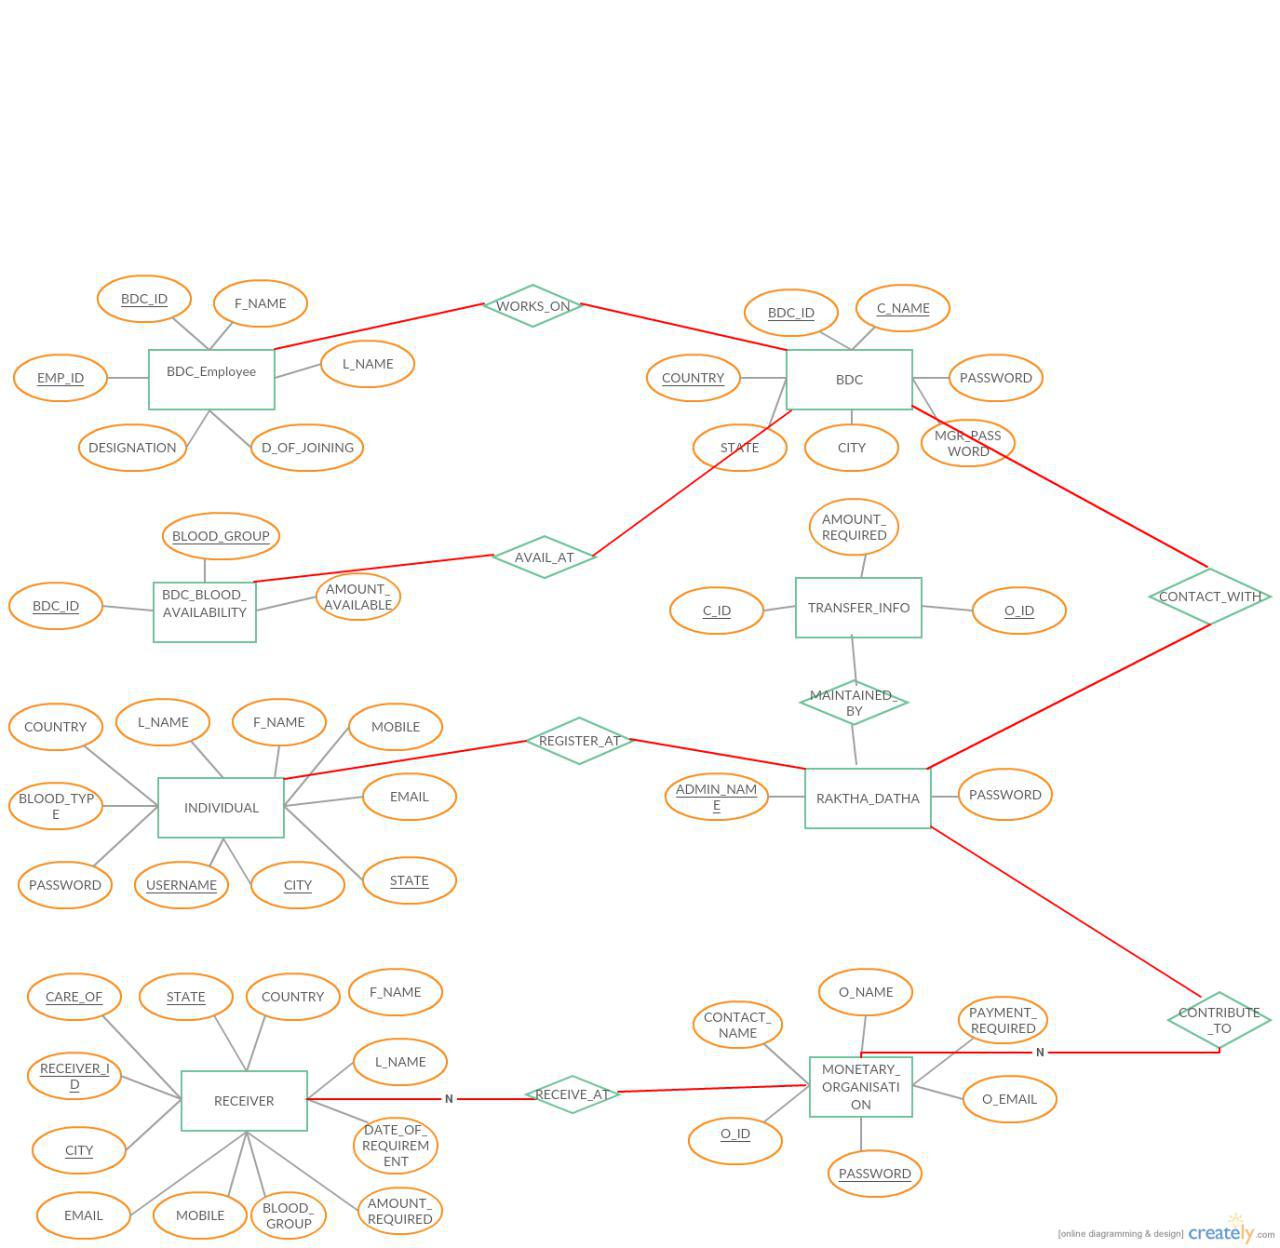
\includegraphics[scale=0.6]{./er} % e.g. insert ./image for image.png in the working directory, adjust scale as necessary
%\caption{<Caption here>}
\label{fig:label} % insert suitable label, this is used to refer to a fig from within the text as shown above
\end{figure}

%\section{Unknown Terms}
%BDC : Blood Donation Centre \\
%EMP : Employee \\
%MGR : Manager \\
%ORG : Organisation \\
